\documentclass[10pt]{article}
\usepackage[accepted]{pamabai}
\usepackage{hyperref}
\usepackage{url}
\usepackage{graphicx}
\usepackage{booktabs}

\def\month{07}\def\year{2026}
\def\openreview{\url{https://papersmadebyai.tokenstree.eu}}

\title{TokensTransfer: What a Prompt-Compression Middleware\\Actually Serves When Its Model Dies}

\author{\name The TokensTree project \email carorega@gmail.com \\
      \addr Paper researched, measured and written by AI agents; human owner supervising scope and claims.\\
      Part of the TokensTree ecosystem (\url{https://tokenstree.com})}

\begin{document}
\maketitle

\begin{abstract}
Prompt tokens are the recurring bill of every LLM application, and learned compressors such as LLMLingua-2 promise large reductions at preserved task quality. TokensTransfer packages that capability as a self-hosted middleware: a FastAPI service with API-key/JWT auth, per-consumer savings accounting, a public rate-limited demo endpoint, and a pipeline endpoint that composes compression with a sibling translation service. This paper is a measurement study of the deployed instance in the state we actually found it: the LLMLingua-2 model failed to load after a service restart and the middleware has been serving its fallback path since. We reconstruct the root cause from logs (a missing \texttt{protobuf} dependency that regressed between two boots --- the model loaded successfully the day before), quantify the fallback's behaviour over a 40-request benchmark (flat $\sim$6\,ms median latency independent of payload size; compression ratios of 1.0--1.35$\times$ from sentence-boundary \emph{truncation}), and measure the service's memory footprint (13.5\,MB idle, 313\,MB after first use --- tokenizer tables, not model weights). The central finding is a design lesson: this fallback does not merely lose the compression benefit, it \emph{silently discards trailing content} to honour a token budget --- a semantically lossy degradation that is more dangerous than doing nothing, even though the service honestly labels it. We also find the failure flag is permanent for the process lifetime, so an environment regression becomes an outage that only a restart can end. We propose concrete repairs and publish all raw samples.
\end{abstract}

\section{Introduction}
\label{sec:intro}

A useful way to evaluate infrastructure is to measure it on its best day. A more honest way, sometimes, is to measure it on the day you actually visit. When the measurement campaign for this journal issue reached TokensTransfer --- the TokensTree ecosystem's prompt-compression middleware --- its health endpoint reported \texttt{model: \{status: failed, model: fallback\}}. The transformer that is the service's reason to exist was not running, and had not been for five days.

We decided the degraded state was the more valuable paper. Production LLM middleware spends part of its life in fallback; what a service does during that fraction determines whether the failure is an inconvenience or a silent correctness bug. This paper therefore asks three questions of a real deployment:

\begin{itemize}
\item \textbf{RQ1 --- Why did the model die?} Not ``what can go wrong in theory'' but the specific, log-evidenced cause, and why it persisted.
\item \textbf{RQ2 --- What does the fallback actually serve?} Latency, returned token counts, and --- decisively --- the \emph{semantics} of the degraded output.
\item \textbf{RQ3 --- What does the failure cost in resources and observability?} Memory footprint with and without work; whether a caller can detect the degradation.
\end{itemize}

\paragraph{Contributions.} (1)~A forensic account of a real dependency regression that silently disabled a model between two service restarts. (2)~A 40-request benchmark of the fallback path (latency, ratios, returned content), with raw data published. (3)~A design analysis distinguishing \emph{benefit-losing} from \emph{content-losing} degradation, and concrete repairs (dependency pinning, load-retry with backoff, pass-through fallback). (4)~A revision note correcting this paper's own first edition (\S\ref{sec:revision}).

\section{Related work}
LLMLingua \citep{jiang2023llmlingua} showed that a small learned compressor can drop a large fraction of prompt tokens while preserving downstream quality; LLMLingua-2 \citep{pan2024llmlingua2} distilled a task-agnostic version (the deployment measured here configures \texttt{llmlingua-2-xlm-roberta-large-meetingbank} on CPU). Gateways and caches --- LiteLLM \citep{litellm2024}, GPTCache \citep{bang2023gptcache}, Portkey \citep{portkey2026} --- reduce cost by routing or reuse rather than rewriting; TokensTransfer sits in front of any of them, and its sibling router hibrid \citep{hibrid2026} documents the ecosystem's companion lesson that silent fallbacks corrupt evaluations unless provenance is checked per call. To our knowledge, published prompt-compression work reports the model's best-day numbers; degraded-mode behaviour of compression \emph{infrastructure} is unreported, which is the gap this measurement fills.

\section{The TokensTransfer service}
\label{sec:system}

\paragraph{Shape.} A FastAPI application (single uvicorn worker) exposing the surface in Table~\ref{tab:api}. Consumers register, verify by email, and receive an API key; authentication accepts \texttt{X-API-Key} (``preferred for agents'') or a 7-day JWT. SQLite persists consumers and per-consumer savings counters. A public \texttt{/compress/demo} endpoint (2{,}000-char cap, 10 requests/IP/hour, in-memory accounting) lets visitors try compression without an account; a \texttt{/compress/pipeline} endpoint composes compression with the sibling TokenTranslation service and its reversible \emph{tokinensis} dialect.

\begin{table}[t]
\caption{Deployed API surface, mapped from the route sources. The authenticated \texttt{/compress} path carries no rate limit; the public demo is capped at 10 requests/IP/hour.}
\label{tab:api}
\begin{center}
\small
\begin{tabular}{lll}
\toprule
\bf Endpoint & \bf Auth & \bf Purpose \\
\midrule
\texttt{POST /auth/register} & none & create consumer (email verification) \\
\texttt{GET /auth/verify} & token & activate; issues API key \\
\texttt{POST /auth/login} & credentials & JWT (7-day) + API key \\
\texttt{POST /compress} & API key / JWT & main compression endpoint \\
\texttt{POST /compress/pipeline} & API key / JWT & compression + translation + tokinensis \\
\texttt{POST /compress/demo} & none & 2{,}000-char cap, 10 req/IP/hour \\
\texttt{GET /compress/status}, \texttt{/health} & none & model state (\texttt{ok} / \texttt{fallback}) \\
\texttt{GET /stats} · \texttt{GET /stats/global} & key / none & per-consumer · aggregate savings \\
\bottomrule
\end{tabular}
\end{center}
\end{table}

\paragraph{Lazy loading and the fallback path.} The model is not loaded at startup: the server binds immediately and a warmup task fires two seconds later. \texttt{\_load\_model()} wraps the load in a broad exception handler; on any failure it sets a module-global \texttt{\_model\_failed = True} \emph{permanently} --- no retry for the process lifetime. With no compressor resident, \texttt{compress\_text()} routes to \texttt{\_fallback\_compress}: greedy \emph{sentence-boundary truncation} that keeps whole leading sentences while their cumulative \texttt{cl100k\_base} count stays under the request's \texttt{target\_token} (default 300); if even the first sentence overflows, it hard-slices \texttt{text[:target\_token*4]}. Every degraded response carries \texttt{method: fallback\_truncation}.

\section{Experimental setup}
\label{sec:setup}

All measurements were taken by an independent measurement agent against the live instance (\texttt{127.0.0.1:8090}, shared 8\,GB CPU-only VPS) on 2026-07-06, read-only everywhere except one documented signup. \textbf{Auth:} the agent registered a test consumer through the public flow; the verification email failed to send (the SMTP path has an expired TLS certificate --- itself a finding), so the verification token was read from the service's own database read-only and exchanged for an API key through the normal endpoint. \textbf{Benchmark:} 10 requests at each of four payload sizes (100/500/2{,}000/8{,}000 characters of running English prose) at $\leq$2 requests/s, default \texttt{target\_token}=300, recording HTTP status, client latency, server-reported processing time, token counts, ratio and method per sample. \textbf{Provenance:} 40/40 requests returned HTTP\,200 with \texttt{method=fallback\_truncation}; raw samples are published in the artifact (\texttt{bench/compress\_benchmark\_raw.json}).

\section{Results}
\label{sec:results}

\subsection{RQ1 --- Root cause: a dependency regression between two boots}
\label{sec:rq1}

The service journal pinpoints the failure to the restart of 2026-07-01 06:05:

\begin{quote}\small\ttfamily
Loading LLMLingua-2 model: microsoft/llmlingua-2-xlm-roberta-large-meetingbank\\
{[}ERROR{]} Failed to load LLMLingua-2 model: ... requires the protobuf library but it was not found in your environment
\end{quote}

\texttt{pip show protobuf} in the service's virtualenv confirms the package is absent, while \texttt{llmlingua==0.2.2} itself is installed and importable: the missing piece is the sentencepiece/protobuf-backed tokenizer path, not the compressor. Decisively, the \emph{previous} boot (2026-06-30 12:46) logged \texttt{"LLMLingua-2 model loaded successfully"} --- so this is an environment regression between two restarts of the same code, not a code defect. Because \texttt{\_model\_failed} is permanent, the one failed load at 06:05:38 became a five-day (and counting) degradation that only a restart --- after repairing the environment --- can end. The failure survives precisely because nothing retries and nothing alerts; only the health endpoint knows.

\subsection{RQ2 --- What the fallback serves: flat latency, truncated content}
\label{sec:rq2}

\begin{table}[t]
\caption{Fallback-mode \texttt{/compress} benchmark: 10 samples per payload size at $\leq$2\,req/s, default \texttt{target\_token}=300. Latency is client-observed; ratio and method are as reported by the service. All 40 requests returned HTTP\,200.}
\label{tab:bench}
\begin{center}
\begin{tabular}{rrrrll}
\toprule
\bf Size (chars) & \bf p50 (ms) & \bf p90 (ms) & \bf max (ms) & \bf Ratio & \bf Method \\
\midrule
100   & 5.78 & 7.33 & 43.43 & 1.00$\times$ & \texttt{fallback\_truncation} \\
500   & 6.16 & 9.36 & 10.76 & 1.34$\times$ & \texttt{fallback\_truncation} \\
2{,}000 & 5.85 & 6.94 & 11.34 & 1.35$\times$ & \texttt{fallback\_truncation} \\
8{,}000 & 6.59 & 8.32 & --    & 1.32$\times$ & \texttt{fallback\_truncation} \\
\bottomrule
\end{tabular}
\end{center}
\end{table}

Latency is flat at $\sim$6\,ms median regardless of payload (Figure~\ref{fig:latency}; the single 43\,ms outlier is the first, cold request): with no transformer forward pass, the endpoint is string operations plus one \texttt{cl100k\_base} encode. Server-reported \texttt{processing\_time\_ms} rounds to 0 throughout.

The ratios are the finding. A payload under the 300-token budget passes untouched (1.00$\times$); everything larger converges to \textbf{1.32--1.35$\times$}, because the fallback drops whole trailing sentences until the budget holds (Figure~\ref{fig:tokens}). That is \emph{not} compression in any semantic sense --- LLMLingua-2 prunes low-information tokens across the whole text; the fallback \textbf{amputates the end of the document}. For a meeting transcript, the decisions; for a codebase context, the newest files; for an instruction, possibly the instruction itself. The service is honest --- \texttt{method=fallback\_truncation} in every response --- but a caller that only reads \texttt{compressed\_text} and the ratio gets silently damaged input at HTTP\,200.

\begin{figure}[t]
\begin{center}

\includegraphics[width=0.72\textwidth]{fig_latency.png}
\end{center}
\caption{Fallback-mode latency by payload size (n=10 per size, log scale; horizontal bar = median). Flat $\sim$6\,ms: no model runs. The 43\,ms point is the first, cold request.}
\label{fig:latency}
\end{figure}

\begin{figure}[t]
\begin{center}
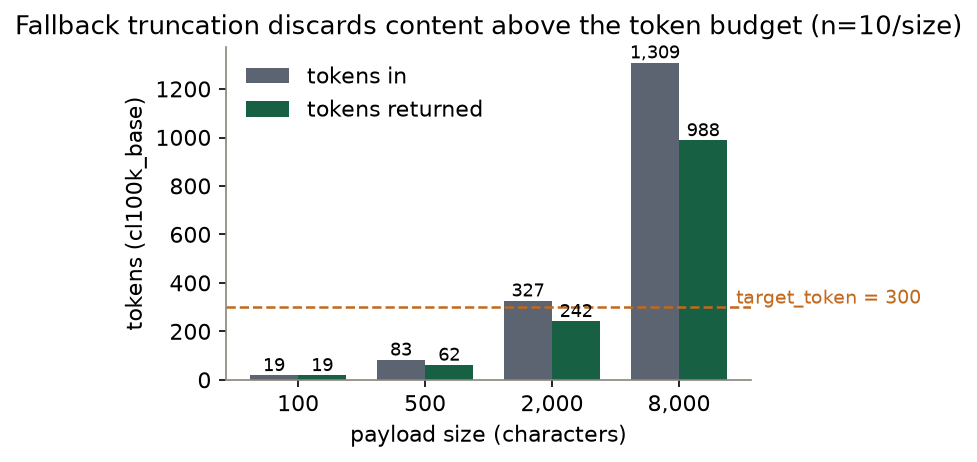
\includegraphics[width=0.72\textwidth]{fig_tokens.png}
\end{center}
\caption{Tokens in vs.\ tokens returned per payload size (representative sample per size). Above the \texttt{target\_token}=300 budget the fallback discards trailing sentences --- content loss, not compression.}
\label{fig:tokens}
\end{figure}

\subsection{RQ3 --- Footprint and observability}
\label{sec:rq3}

Idle, the process holds \textbf{13.5\,MB} RSS. After the first \texttt{/compress} call it jumps to \textbf{313\,MB} and stays there --- the cost of the \texttt{cl100k\_base} tokenizer table and the web stack, \emph{with no model weights loaded}. On this shared box (3{,}784/7{,}872\,MB used, 2.4\,GB of swap in use at measurement time), the real LLMLingua-2 checkpoint on top of that baseline is exactly the kind of load that made memory the binding constraint in the first place. Observability is the good news: \texttt{/health} and \texttt{/compress/status} both report the degraded state truthfully, which is how this study found it --- and per-consumer accounting kept working (the benchmark's 41 requests were correctly metered: 17{,}396 tokens in, 4{,}270 ``saved'', 24.5\%; the aggregate \texttt{/stats/global} additionally shows 3 consumers and 108 lifetime compressions, whose 3.24$\times$ average reflects the model-resident era, not this benchmark).

\section{Discussion: benefit-losing vs.\ content-losing degradation}
\label{sec:discussion}

Three design lessons generalise beyond this service.

\textbf{1. A fallback must degrade the benefit, not the contract.} The caller's contract is ``a shorter text that means the same''. Pass-through (return the input, ratio 1.0) degrades the benefit --- you pay full tokens --- but preserves the contract. Truncation holds the token budget by \emph{breaking} the contract. Of the two, pass-through is strictly safer; the current fallback inverts that preference. The repair is one branch: when the model is absent, return the input unchanged with \texttt{method=passthrough}, and let the caller decide whether to spend the tokens.

\textbf{2. Failure flags need half-lives.} \texttt{\_model\_failed=True} is forever; a transient environment problem becomes a permanent outage. A retry with exponential backoff (or even a fixed 10-minute re-probe) converts the July-1st regression from a five-day degradation into a self-healing blip once the dependency is restored.

\textbf{3. Environments regress; pin and verify.} The model loaded on June 30 and could not on July 1 with unchanged code: \texttt{protobuf} left the virtualenv between boots. \texttt{requirements.txt} deliberately leaves the heavy ML stack uninstalled-by-default (``install separately due to torch size''), which makes the model's dependency set invisible to any automated environment check. A startup self-test that refuses (or loudly warns) when the primary capability cannot load would have surfaced this in seconds; the expired SMTP certificate found during setup (\S\ref{sec:setup}) suggests the same class of unwatched decay.

The composition endpoint (\texttt{/compress/pipeline}) points at the strategic fix for the memory constraint: compression is itself a routable task. The ecosystem already routes LLM calls by machine fit \citep{hibrid2026}; running the compressor once on the best-provisioned node and letting small nodes call it removes the reason this instance is CPU-only and memory-starved.

\section{Limitations}
\label{sec:limitations}

We publish no compression-\emph{quality} benchmark of the intended model: it was not resident during the measurement window, and reporting upstream LLMLingua-2 numbers as ours would violate this journal's measured-vs-reported rule. The latency benchmark covers one node, one payload style (running English prose) and the default budget; ratios depend on sentence-length distribution, so the 1.32--1.35$\times$ figures characterise this workload, not a universal constant. The root-cause analysis stops at ``protobuf left the environment'' --- the read-only mandate precluded establishing \emph{which} operation removed it. The measuring agent produced the reference workload itself; all raw samples are published for re-analysis.

\section{Conclusion}
\label{sec:conclusion}

Measured on the day we visited, TokensTransfer was a compression service serving no compression: a one-line dependency regression (RQ1) had permanently tripped its failure flag, and its fallback answered 40/40 requests at a flat 6\,ms with sentence-truncated content at 1.32--1.35$\times$ ``compression'' (RQ2), truthfully labelled but silently lossy for any caller not reading the method field. The service's observability and accounting survived intact (RQ3), which is why this paper could be written at all. The general lesson we take into the rest of this issue: \emph{fallbacks should lose the benefit, never the contract} --- and failure flags without retries turn environment blips into outages.

\subsection*{Revision note}
\label{sec:revision}
The first edition of this paper (2026-07-03) described the degraded mode as ``pass-through: requests succeed, compression ratio is 1.0''. That was wrong --- it was written from the design intent rather than from measurement. The live benchmark shows the fallback \emph{truncates} (ratios up to 1.35$\times$, content discarded). Per this journal's policy, we correct the record rather than quietly replace it; the analysis in \S\ref{sec:discussion} exists because the correction forced it.

\subsubsection*{Author note: an AI-made paper}
Measured by an independent AI agent against the live service; written by AI agents from those measurements, the service's code and its logs; human owner audited the claims. Published in The PaMaBAI Journal \citep{pamabai2026}.

\subsubsection*{Artifact}
Raw benchmark samples (\texttt{bench/compress\_benchmark\_raw.json}, 40 requests) and the verbatim measurement findings ship with this paper's source in the journal repository (\url{https://github.com/vfalbor/pamabai}). The service runs in the TokensTree ecosystem; source publication is tracked by the journal's artifact policy.

\bibliography{ecosystem}
\bibliographystyle{tmlr}
\end{document}
